\chapter{Конструкторский раздел}

В данном разделе изучаются индексы, типы индексов, индексы в СУБД MySQL. На основе этой информации описывается алгоритм построения индексов для сложных запросов. Данная задача рассматривается по объектно-ориентированной методологии. 

\section{Индексы}

Индекс — объект базы данных, создаваемый с целью повышения производительности поиска данных. Таблицы в базе данных могут иметь большое количество строк, которые хранятся в произвольном порядке, и их поиск по заданному критерию путём последовательного просмотра таблицы строка за строкой может занимать много времени. Индекс формируется из значений одного или нескольких столбцов таблицы и указателей на соответствующие строки таблицы и, таким образом, позволяет искать строки, удовлетворяющие критерию поиска. Ускорение работы с использованием индексов достигается в первую очередь за счёт того, что индекс имеет структуру, оптимизированную под поиск.

\paragraph{Производительность}
\label{paragraph:performance}

Для оптимальной производительности запросов индексы обычно создаются на тех столбцах таблицы, которые часто используются в запросах. Для одной таблицы может быть создано несколько индексов. Однако увеличение числа индексов замедляет операции добавления, обновления, удаления строк таблицы, поскольку при этом приходится обновлять сами индексы. Кроме того, индексы занимают дополнительный объем памяти, поэтому перед созданием индекса следует убедиться, что планируемый выигрыш в производительности запросов превысит дополнительную затрату ресурсов компьютера на сопровождение индекса. \cite{wikipedia.org:index}

Существует много типов индексов, каждый из которых лучше всего подходит для достижения той или иной цели. Индексы реализуются на уровне подсистем хранения, а не на уровне сервера. Таким образом, они не стандартизованы: в каждой подсистеме индексы работают немного по-разному, и далеко не все подсистемы допускают использование существующего разнообразия индексов. Даже если некоторый тип поддерживается в нескольких подсистемах хранения, внутренняя реализация может различаться. \cite{zaitsev} 

Поэтому для начала рассмотим какие подсистемы хранения реализованы в MySQL,
 а затем некоторые типы индексов.  


\section{Подсистемы хранения MySQL}

При разработке приложения для MySQL необходимо решить, какую подсистему хранения использовать. Поскольку допустимо выбирать способ хранения данных для каждой таблицы в отдельности, нужно ясно понимать, как будет использоваться каждая таблица, и какие данные в ней планируется хранить. Это также поможет получить хорошее представление о приложении в целом и о потенциале его роста. Вооружившись этой информацией, можно осознанно выбирать подсистемы хранения данных.

Согласно \cite{tagline.ru:List_DBMS} самые распространенные подсистемы хранения: MyISAM — 74,4\%, InnoDB — 68,5\%, другие движки — 31\%. В связи с тем, что один и тот же тип индекса в разных подсистемах хранения может быть реализован по-разному, они будут иметь свои приемущества и недостатки. \cite[p.~137]{zaitsev}

\subsection{Подсистема MyISAM}

Как одна из самых старых подсистем хранения, включенных в MySQL, MyISAM обладает многими функциями, которые были разработаны за годы использования СУБД для решения различных задач. Она предоставляет полнотекстовое индексирование, сжатие и пространственные функции (для геоинформационных систем – ГИС). MyISAM не поддерживает транзакции и блокировки на уровне строк.


\subsection{Подсистема InnoDB}

Подсистема хранения InnoDB была разработана для транзакционной обработки, в частности для обработки большого количества краткосрочных транзакций, которые значительно чаще благополучно завершаются, чем откатываются. Она остается наиболее популярной транзакционной подсистемой хранения. Высокая производительность и автоматическое восстановление после сбоя делают ее популярной и для нетранзакционных применений.



\section{Типы индексов}

\subsection{B-tree-индексы}

Когда говорят об индексе без упоминания типа, обычно имеют в виду B-Tree индексы, в которых для хранения данных используется структура, называемая B-tree. Во многих подсистемах хранения на самом деле используются индексы типа B+Tree, в которых каждый листовой узел содержит указатель на следующий для ускорения обхода дерева по диапазону значений.

Общая идея B-дерева заключается в том, что значения хранятся по порядку, и все листовые страницы находятся на одинаковом расстоянии от корня. На рисунке \ref{img:btree-structure} показано абстрактное представление B-Tree индекса. B-Tree-индекс ускоряет доступ к данным, поскольку подсистеме хранения не нужно сканировать всю таблицу для поиска нужной информации. Вместо этого она начинает с корневого узла (не показанного на этом рисунке). В корневом узле имеется массив указателей на дочерние узлы, и подсистема хранения переходит по этим указателям. Чтобы найти подходящий указатель, она просматривает значения в узловых страницах, которые определяют верхнюю и нижнюю границы значений в дочерних узлах. В конечном итоге подсистема хранения либо определяет, что искомое значение не существует, либо благополучно достигает листовой страницы.

Поскольку в B-Tree индексах индексированные столбцы хранятся в упорядоченном виде, то они полезны для поиска по диапазону данных. Например, при спуске вниз по дереву индекса, построенного по текстовому полю, значения перебираются в алфавитном порядке, поэтому поиск «всех лиц, чьи фамилии начинаются с буквы от В до Д» оказывается эффективным.

\begin{figure}[H]
  \centering
  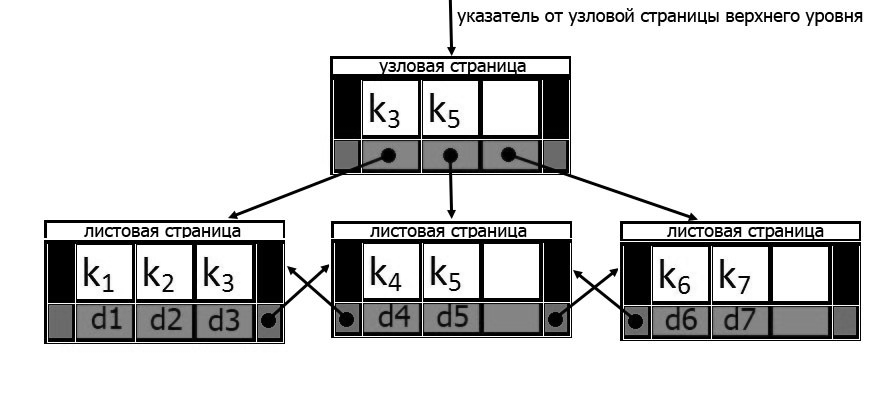
\includegraphics[scale=0.5]{btree.png}
  \caption{Структура данных B+tree.}
  \label{img:btree-structure}
\end{figure}

Где $k_i$ - ключи ($k_i < k_i + 1$), $d_i$ - данные.

Сложность поиска в линейной структуре данных $O(N)$, а в B-tree $O(log(k)+N_k$), где $k$ — количество уровней, а $N_k$ — количество элементов в узле. Поэтому индексы, использующие структуру данных B-tree, эффективны для поиска данных. 

Подсистемы хранения представляют B-Tree-индексы на диске по-разному, и это может влиять на производительность. Например, в MyISAM используется техника сжатия префикса, позволяющая уменьшить размер индекса, а InnoDB не сжимает индексы, поскольку это лишило бы ее возможности выполнять некоторые оптимизации. Кроме того, индексы MyISAM ссылаются на индексированные строки по их физическому адресу на диске, а InnoDB – по значениям первичного ключа. Каждый вариант имеет свои достоинства и недостатки.

\subsection{Хеш-индексы}

Хеш-индекс строится на основе хеш-таблицы и полезен только для точного поиска с указанием всех столбцов индекса. Для каждой строки подсистема хранения вычисляет хеш-код индексированных столбцов – сравнительно короткое значение, которое, скорее всего, будет различно для строк с разными значениями ключей. В индексе хранятся хеш-коды и указатели на соответствующие строки. Т.е. хеш-индексы предполагают хранение не самих значений, а их хэшей, благодаря чему уменьшается размер (а, соответственно, и увеличивается скорость их обработки) индексов из больших полей. Таким образом, при запросах с использованием хеш-индексов, сравниваться будут не искомое со значения поля, а хэш от искомого значения с хэшами полей. 

Из-за нелинейнойсти хэш-функций данный индекс нельзя сортировать по значению, что приводит к невозможности использования в сравнениях больше/меньше и «is null». Кроме того, так как хэши не уникальны, то для совпадающих хэшей применяются методы разрешения коллизий.

Подсистема хранения InnoDB поддерживает так называемые адап­тивные хеш-индексы. Когда InnoDB замечает, что доступ к некоторым значениям индекса происходит очень часто, она строит для них хеш-индекс в памяти, помимо уже имеющихся B-Tree-индексов. Тем самым к B-Tree-индексам добавляются некоторые свойства хеш-индексов, например очень быстрый поиск. Этот процесс полностью автоматический, и вы не можете ни контролировать, ни настраивать его.

\subsection{Полнотекстовые индексы}

В большинстве типичных запросов присутствует фраза WHERE, в которой значения сравниваются на равенство, выделяются диапазоны строк и т. д. Но иногда нужно искать по ключевому слову, и в этом случае поиск должен быть основан на релевантности, а не простом сравнении строк. Для этой цели и предназначены системы полнотекстового поиска. Для полнотекстового поиска требуется специальный синтаксис запроса. Индекс необязателен, но при его наличии поиск выполняется быстрее. Полнотекстовые индексы имеют специальную структуру, ускоряющую поиск документов, содержащих заданные ключевые слова.

Полнотекстовый (FULLTEXT) индекс позволяет искать в тексте ключевые слова, а не сравнивать искомое значение со значениями в столбце. Полнотекстовый поиск не имеет ничего общего с другими типами поиска. С ним связано много тонкостей, например стоп-слова, стемминг, учет множественного числа, а также булевский поиск. Он гораздо больше напоминает поисковые системы, нежели обычное сравнение с критерием во фразе WHERE.

В MySQL поддержка полнотекстового поиска реализована только в подсистеме MyISAM.



\section{B-tree индексы в MySQL InnoDB}
\label{section:b-tree-indexes-innodb}

В данной работе рассматриваются только B-tree-индексы для подсистемы хранения InnoDB.

Рассмотрим более подробно B-tree индексы в MySQL InnoDB. В качестве примера возьмем таблицу \ref{tabular:poets}, заголовок которой $poet (poet\_id, last\_name, first\_name, dob, country)$

\begin{table}[h]
\caption{Таблица поэтов}
\label{tabular:poets}
\medskip
\begin{tabular}{|l|l|l|l|l|}
\hline
poet\_id & last\_name & first\_name & dob & country\\
\hline
1 & "Блок" & "Александр" & 1880 & "ru"\\
2 & "Фет" & "Афанасий" & 1820 & "ru"\\
3 & "Лермонтов" & "Михаил" & 1814 & "ru"\\
4 & "Ильф" & "Илья" & 1897 & "ru"\\
5 & "Пушкин" & "Александр" & 1799 & "ru"\\
6 & "Булгаков" & "Михаил" & 1891 & "ru"\\
7 & "Есенин" & "Сергей" & 1895 & "ru"\\
\hline
\end{tabular}
\end{table}

\subsection{Кластерный индекс}

В InnoDB данные хранятся в структуре данных B+tree, где в узловых страницах хранятся первичные ключи, а в листовых страницах хранятся данные. Такое дерево называется кластерным индексом. Над таблицей можно построить только один кластерный индекс, поскольку невозможно хранить одну и ту же запись одновременно в двух местах. Однако часть или всю запись можно хранить в нескольких местах, что будет использоваться в покрывающих индексах \ref{section:covering-index}.

Для рисунка \ref{img:btree-structure} и таблицы \ref{tabular:poets}: $k_1 \ldots k_7$ - первичные ключи ($poet\_id$), $k_i = i$, $d_1 \ldots d_7$ - данные, т.е. $d_1$ = Блок, Александр, 1880, ru; $d_2$ = Фет, Афанасий, 1820, ru; $\ldots$


\subsection{Вторичный индекс}

Для оптимизации конкретных запросов используются \textit{вторичные индексы} (далее просто индексы). В узловых страницах индексов хранятся поля, по которым создан этот индекс, а в листовых страницах хранится значение первичного ключа. Для каждой таблицы в одном запросе используется только один индекс. При использовании в запросах индекса, сначала будет найдено значение первичного ключа, затем по этому значению будут найдены данные в кластерном индексе. Поэтому при создании вторичного индекса, в конец неявно добавляется первичный ключ.

На рисунке \ref{img:index-structure} показан индекс по полю \textit{(dob)}: $k_1 \ldots k_7$ - ключи, по которым построен индекс; $k_1$ = 1799, $k_2$ = 1814, $k_3$ = 1820, $\ldots$; $p_1 \ldots p_7$ - первичные ключи ($poet\_id$); $p_i = i$.

\begin{figure}[H]
  \centering
  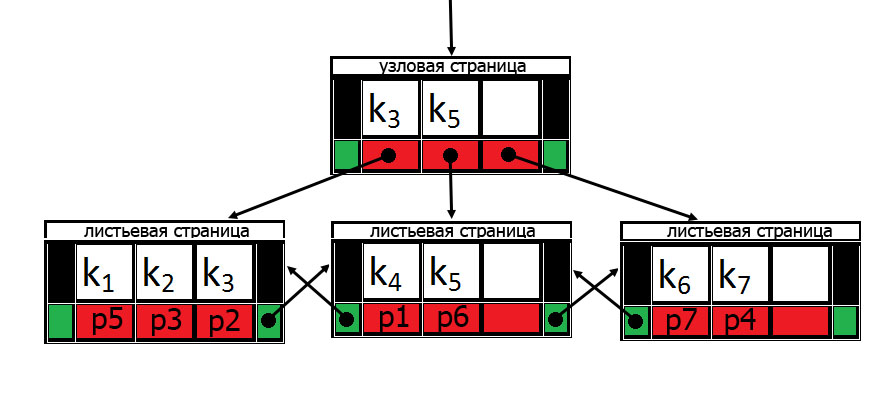
\includegraphics[scale=0.6]{index-structure.png}
  \caption{Структура вторичного индекса}
  \label{img:index-structure}
\end{figure}


\subsection{Составной индекс}

\textit{Составной индекс} - это индекс, построенный по нескольким полям. Чтобы правильно использовать составные индексы, необходимо понять структуру их хранения. Все работает точно так же, как и для обычного индекса, но для значений используются значения всех входящих колонок сразу, по которым строится индекс.

Если построить индекс по полям \textit{(dob, last_name)}, то для рисунка \ref{img:index-structure} $k_1$ = 1799Пушкин, $k_2$ = 1814Лермонтов, $k_3$ = 1820Фет, $\ldots$

\subsection{Частичный индекс}

\textit{Составной индекс} может использоваться не полностью, но только как левый префикс. Такое использование индекса наызвается \textit{частичным индексом}. 

Оператор \textit{LIKE} с использованием знака \% в конце указываемого шаблона рассматривается как левый префикс.

\subsection{Селективность индексов}

Чем меньше строк войдет в выборку, тем быстрее будет работать поиск по ней. Индекс, дающий наименьшую выборку, называется \textit{более селективным}. Если СУБД может применить несколько индексов к данному SQL запросу, то использоваться будет более селективный.

\subsection{Покрывающий индекс}
\label{section:covering-index}

Индекс называется \textit{покрывающим}, если в нем есть все поля, используемые в запросе. Для того чтобы вернуть результат запроса при использовании покрывающего индекса СУБД не нужно обращаться к кластерному индексу. Покрывающие индексы позволяют имитировать кластерные индексы. 

Для запроса на листинге \ref{sql:covering-index} можно построить индекс $(last\_name, dob)$, который будет считаться покрывающим.
\begin{lstlisting}[language=sql, label=sql:covering-index, caption={запрос для covering-index}]
SELECT last_name, dob
FROM poet
WHERE last_name = "Пушкин"
\end{lstlisting}



\section{Индексы для сложных запросов}


\paragraph{Общие правила}

\begin{enumerate}
\item в одном запросе для каждой таблицы используется максимум один индекс;
\item в выражениях \textit{GROUP BY} и \textit{ORDER BY} поля только из одной таблицы.
\end{enumerate}


Под \textit{сложным запросом} будем понимать запросы, вида листинг \ref{view-join-query}.

\begin{lstlisting}[language=sql, caption={Вид сложного запроса},label=view-join-query]
SELECT * FROM
t1 {INNER | LEFT | RIGHT} JOIN t2 ON conditional_definition
    [WHERE where_definition]
    [ORDER BY col_name [ASC | DESC]]

where_definition:
    where_expression or 
    where_expression [AND] where_expression 
    
where_expression:
    column_name [> | >= | = | <> | <= | < ] constant or
    column_name LIKE constant or 
    where_definition   

conditional_definition:
    conditional_expression or 
    conditional_expression [AND] conditional_expression 

conditional_expression:
    column_name = column_name or
    conditional_expression
\end{lstlisting}

\section{Определение индексов для сложных запросов}

На рисунках \ref{img:idef0-all-process}, \ref{img:idef0-all-process-detail}, \ref{img:full-alg} представлена последовательность действий для определения индексов, рекомендуемых для \textit{сложного запроса}.


\begin{figure}[h!]
  \centering
  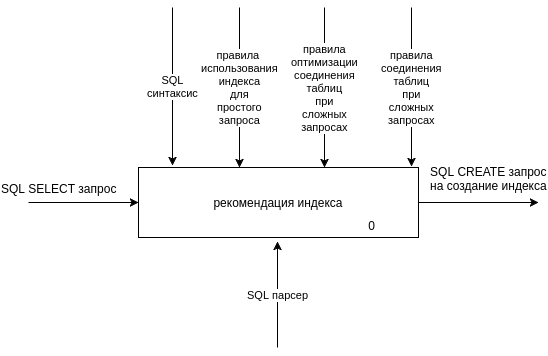
\includegraphics[scale=0.7]{idef0-all-process.png}
  \caption{Диаграмма IDEF0 определения рекомендуемых индексов для сложного запроса}
  \label{img:idef0-all-process}
\end{figure}

\begin{figure}[h!]
  \centering
  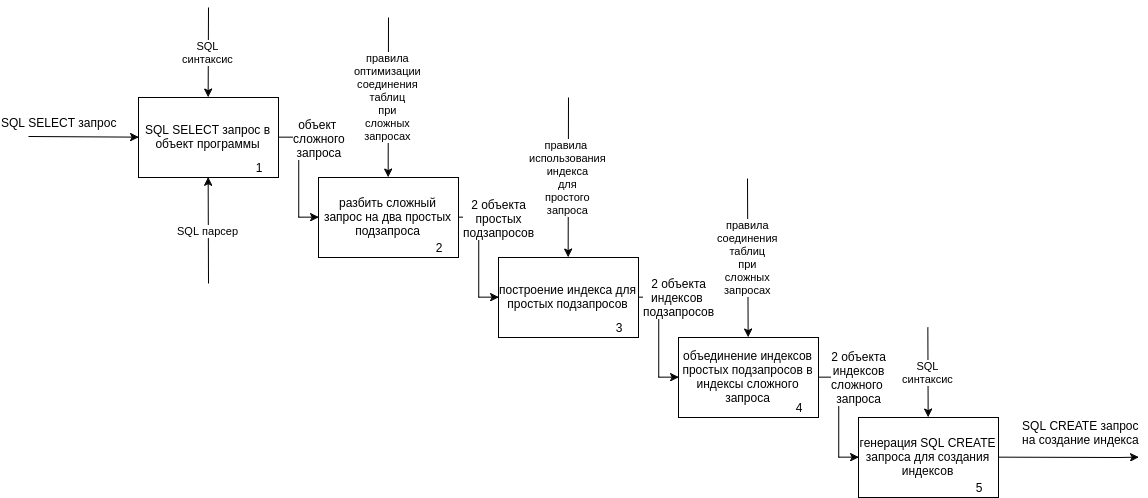
\includegraphics[scale=0.4]{idef0-all-process-detail.png}
  \caption{Диаграмма IDEF0 определения рекомендуемых индексов для сложного запроса (декомпозиция)}
  \label{img:idef0-all-process-detail}
\end{figure}

\begin{figure}[h!]
  \centering
  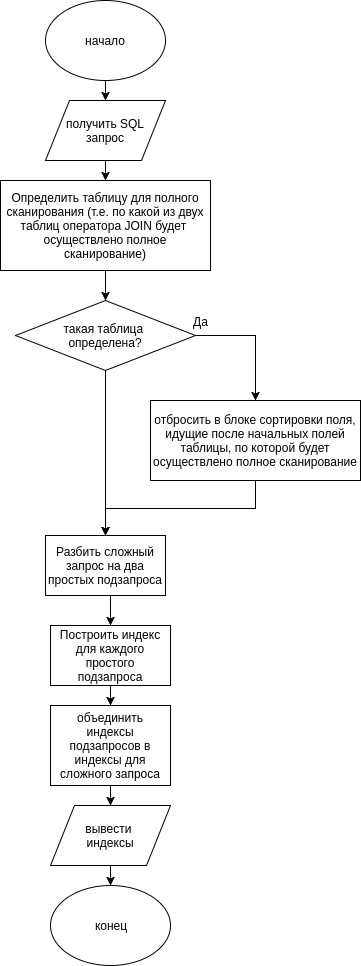
\includegraphics[scale=0.5]{full-alg.png}
  \caption{Схема определения рекомендуемых индексов для сложного запроса}
  \label{img:full-alg}
\end{figure}

\indent
Опишем некоторые действия более подробно.


\section{Fullscan алгоритм}

При соединении двух таблиц (A и B), для каждой строки одной таблицы A будет происходить сканирование другой таблицы B. Такое сканирование таблицы A назовем \textbf{полным сканированием}. 

\textbf{Fullscan алгоритм} - алгоритм для определения таблицы, по которой будет осуществлено полное сканирование. Алгоритм на вход принимает текст запроса и возвращает название таблицы, по которой будет полное сканирование или null, если таблица не определена (в таком случае MySQL после выбора подходящих индексов выберет, по какой таблице будет происходить полное сканирование).

В качестве fullscan алгоритма для join-запроса можно предложить алгоритм, при работе которого происходит анализ исследуемого запроса. Псевдокод представлена в алгоритме \ref{alg:fullscan}. Блок-схема представлена на рисунке \ref{img:fullscan}.

\begin{algorithm}[h]
\caption{Fullscan алгоритм}\label{alg:fullscan}
\begin{algorithmic}[1]
 
\Function{fullscanAlg}{query}
    \If {условие соединения $A LEFT JOIN B$}
        \If {в условии WHERE исключается возможность равенства любого из полей таблицы B значению null}
            \State {заменить $LEFT JOIN$ на $INNER JOIN$}
        \Else
            \State \Return таблица $A$
        \EndIf
    \EndIf
    \Statex 
    
    \If {условие соединения $A RIGHT JOIN B$}
        \If {в условии WHERE исключается возможность равенства любого из полей таблицы $A$ значению null}
            \State {заменить $RIGHT JOIN$ на $INNER JOIN$}
        \Else
            \State \Return таблица $B$
        \EndIf
    \EndIf
    \Statex 

    \If {условие соединения $A INNER JOIN B$}
        \If {есть сортировка $ORDER BY A.a, \ldots$}
            \State \Return таблица $A$
        \ElsIf {есть сортировка $ORDER BY B.a, \ldots$}
            \State \Return таблица $B$
        \EndIf
    \EndIf
    \Statex 

    \State \Return $null$
\EndFunction
 
\end{algorithmic}
\end{algorithm}

\begin{figure}[h]
  \centering
  \includegraphics[scale=0.5]{fullscan.png}
  \caption{Блок-схема fullscan-алгоритма.}
  \label{img:fullscan}
\end{figure}


\subsection{Примеры работы алгоритма}

Рассмотрим работу fullscan алгоритма по обработке заданного SQL запроса на конкретных практических примерах.

\paragraph{Пример №1}

\begin{lstlisting}[language=SQL]
query = {FROM t1 LEFT JOIN t2 ON t1.a = t2.a WHERE t1.b > 1 AND t2.c = 5}
\end{lstlisting}

Условие соединения - $LEFT JOIN$. В условии $WHERE$ исключается возможность равенства поля $t2.c$ значению $null$, значит изменим запрос на
\begin{lstlisting}[language=SQL]
query = {FROM t1 INNER JOIN t2 ON t1.a = t2.a WHERE t1.b > 1 AND t2.c = 5}
\end{lstlisting}

Условие соединения - $INNER JOIN$. Сортировок нет, значит вернуть $null$. 

\textbf{Ответ:} по какой таблице будет осуществлено полное сканирование на данном этапе не определено.


\paragraph{Пример №2}
\begin{lstlisting}[language=SQL]
query = {FROM t1 LEFT JOIN t2  ON t1.a = t2.a WHERE t1.b = 5000 AND t1.c > 3 ORDER BY t2.c, t2.d}
\end{lstlisting}

Условие соединения - $LEFT JOIN$. В условии $WHERE$ не исключается возможность равенства любого поля таблицы $t2$ значению $null$, значит вернуть $t1$.

\textbf{Ответ:} по таблице $t1$ будет осуществлено полное сканирование. 


\paragraph{Пример №3}
\begin{lstlisting}[language=SQL]
query = {FROM t1 LEFT JOIN t2 ON t1.a = t2.a WHERE t2.b = 5000 AND t2.c > 3 ORDER BY t2.c, t2.d}
\end{lstlisting}

Условие соединения - $LEFT JOIN$. В условии $WHERE$ исключается возможность равенства поля $t2.b$ и $t2.c$ значению $null$, значит изменим запрос на
\begin{lstlisting}[language=SQL]
query = {FROM t1 INNER JOIN t2 ON t1.a = t2.a WHERE t2.b = 5000 AND t2.c > 3 ORDER BY t2.c, t2.d}
\end{lstlisting}

Условие соединения - $INNER JOIN$. Есть сортировка $ORDER BY t2.c, \ldots$. Вернуть $t2$.

\textbf{Ответ:} по таблице $t2$ будет осуществлено полное сканирование. 


\subsection{Отбрасывание лишних полей в блоке сортировки}

Необходимо отбросить в блоке сортировки поля, идущие после начальных полей таблицы, по которой будет осуществлено полное сканирование.

\paragraph{Примеры}

Пусть\\
\textit{T = t2},\\
\textit{query = $\ldots$ ORDER BY t2.z, t2.y, t1.z, t1.y, t2.x $\ldots$},\\
тогда \\
\textit{query1 = $\ldots$ ORDER BY t2.z, t2.y}

Пусть \\
\textit{T = t2},\\
\textit{query = $\ldots$ ORDER BY t1.x, t2.x $\ldots$},\\
тогда отбрасываются все поля (т.е. в \textit{query1} не будет сортировки)


\subsection{Разбиение сложного запроса}

Сложный запрос необходимо разбить на два простых подзапроса, при этом в условии соединения таблиц отбрасываемую таблицу заменить на \textit{CONST} и переместить в блок \textit{WHERE}.

\paragraph{Примеры}

Пусть \\
\textit{query = $\ldots$ ON t1.a = t2.a WHERE t1.b = Z, t2.b = Y $\ldots$},\\
тогда\\
\textit{query1 = $\ldots$ WHERE t1.a = CONST AND t1.b = Z $\ldots$}, \\
\textit{query2 = $\ldots$ WHERE t2.a = CONST AND t2.b = Y $\ldots$}


\subsection{Построение индекса для простого запроса}

Для того, чтобы автоматизировать процесс построения индекса, рассмотренные в разделе \ref{section:b-tree-indexes-innodb}, необходимо исследовать в каких случаях они могут применяться. Рассмотрим примеры использования индексов для простых запросов (по одной таблице).


\paragraph{Индексы для WHERE}

Для запроса на листинге \ref{sql:index-on-where} можно построить индексы \textit{(dob, last\_name)} и \textit{(last_name, dob)}.
\begin{lstlisting}[language=sql, label=sql:index-on-where, caption={запрос для index-on-where}]
SELECT * 
FROM poet
WHERE last_name = ”Пушкин” 
    AND dob = 1799
\end{lstlisting}

Рассмотрим работу индексов на примере индекса \textit{INDEX $\equiv$ (a, b, c)}, где \textit{a, b} - числа, \textit{c} - строка.

\begin{enumerate}
\item \textit{a = 5 AND b = 10 AND c="Hello world"} \\  \textit{INDEX} применяется полностью
\item \textit{b = 5} \\   \textit{INDEX} не применяется
\item \textit{a = 5} \\  \textit{INDEX} применяется как левый префикс по первому полю
\item \textit{a = 5 AND b = 10} \\  \textit{INDEX} применяется как левый префикс по первым двум полям
\item \textit{a = 5 AND b = 10 AND c LIKE "Hello w\%"}  \\  \textit{INDEX} применяется как левый префикс по первым трем полям
\item \textit{a > 5} \\  \textit{INDEX} применяется как левый префикс по первому полю
\item \textit{a = 5 AND b IN (2,3)} \\ условие \textit{IN} - рассматривается как поиск по диапазону, \textit{INDEX} применяется как левый префикс по первым двум полям
\item \textit{a=5 AND b=10 AND c LIKE "\% world"} \\  \textit{INDEX} применяется как левый префикс по первым двум полям
\item \textit{a>5 AND b=2} \\ \textit{INDEX} применяется как левый префикс по первому полю
\item \textit{a=5 AND c=10} \\ \textit{INDEX} применяется как левый префикс по первым двум полям
\end{enumerate}


\paragraph{Индексы при сортировке}

В индексе данные хранятся в отсортированном виде, поэтому дополнительно сортировать данные выборки не требуется.


Для запроса на листинге \ref{sql:index-order1} строим индекс \textit{(dob)}.

\begin{lstlisting}[language=sql, label=sql:index-order1, caption={запрос для index-order}]
SELECT * 
FROM poet
ORDER BY dob
\end{lstlisting}


Для запроса на листинге \ref{sql:index-order2} строим индекс \textit{(country, dob)}. В индексе находим строки, удовлетворяющие условию \textit{country="ru"}, а в этой выборке строки уже отсортированы по \textit{dob}.

\begin{lstlisting}[language=sql, label=sql:index-order2, caption={запрос для index-order}]
SELECT * 
FROM poet
WHERE country="ru" 
ORDER BY dob
\end{lstlisting}


Для запроса на листинге \ref{sql:index-order3} строим индекс \textit{(dob)}. \textit{GROUP BY} возьмет уже отсортированные строки из индекса и уберет повторы, а т.к. строки уже отсортированные - \textit{ORDER BY} всего лишь задаст, в каком порядке выводить данные. 

\begin{lstlisting}[language=sql, label=sql:index-order3, caption={запрос для index-order}]
SELECT *
FROM poet
GROUP BY dob
ORDER BY dob
\end{lstlisting}


Примеры запросов, к которым применяется индекс \textit{(a, b)}:

\begin{enumerate}
\item сортировка по первой колонке
\item первая колонка в условии \textit{WHERE}, и сортировка по второй колонке
\item первая колонка в условии \textit{WHERE} и сортировка по первой колонке
\item сортировка по двум колонкам и обе в одну сторону
\end{enumerate}


Примеры запросов, к которым не применяется индекс \textit{(a, b)}:

\begin{enumerate}
\item сортировка по второй колонке, при этом в условии \textit{WHERE} первая колонка не проверяется на строгое равенство. Например, для запроса \textit{WHERE a>5 ORDER BY b} в индексе будут данные \textit{(a, b): a=6, b=2; a=6, b=3; a=7, b=0; a=8, b=1}. MySQL сделает выборку по условию \textit{a>5}, но в этой выборке строки не отсортированы по \textit{b}.
\item \textit{WHERE a IN (1,2) ORDER BY b} (аналогично предыдущему запросу)
\item сортировка разных столбцов в разных направлениях\\
Чтобы обойти это, можно сделать виртуальную колонку, например, перед числом поставить минус.
\end{enumerate}



\paragraph{Агрегирующие функции MIN, MAX}

Так как данные в индексе отсортированы, то для нахождения минимального или максимального значения достаточно взять крайнее значение.

Для запроса на листинге \ref{sql:index-aggr1} строим индекс $(dob)$.
\begin{lstlisting}[language=sql, label=sql:index-aggr1, caption={запрос для index-aggr}]
SELECT MAX(dob) 
FROM poet;
\end{lstlisting}

Для запроса на листинге \ref{sql:index-aggr2} строим индекс $(first\_name, dob)$.
\begin{lstlisting}[language=sql, label=sql:index-aggr2, caption={запрос для index-aggr}]
SELECT MAX(dob) 
FROM poet
GROUP BY first_name
\end{lstlisting}




\subsection{Объединение индексов подзапросов}

При объединении индексов для двух простых подзапросов необходимо из индекса для таблицы, по которой будет полное сканирование, удалить поле, по которому происходит соединение таблиц. Если таблица, по которой происходит полное сканирование, не определена, то вернуть две пары индексов, каждая из которых может быть использована для оптимизации выполнения запроса.

Пусть \\
\textit{T = t1},\\
\textit{index(t1) = t1(a, b)},\\
\textit{index(t2) = t2(c, a)},\\
\textit{query0 = $\ldots$ ON t1.a = t2.a $\ldots$},\\
тогда индексы для сложного запроса: \\
\textit{index(t1) = t1(b)}, \textit{index(t2) = t2(c, a)}.

Пусть \\
\textit{T = NULL},\\
\textit{index(t1) = t1(a, b, c)},\\
\textit{index(t2) = t2(a, b, c)},\\
\textit{query1 = $\ldots$ ON t1.a = t2.a $\ldots$},\\
тогда индексы для сложного запроса: \\
\textit{index1(t1) = t1(a, b, c)}, \textit{index2(t2) = t2(b, c)},\\ 
\textit{index2(t1) = t1(b, c)}, \textit{index1(t2) = t2(a, b, c)}.


\section{Объектно-ориентированный анализ}

В реультате анализа можно выделить следующие сущности:

\begin{enumerate}
\item поле
\item аргумент
\item условное выражение
\item выражение блока ON
\item выражение блока ORDER BY
\item простой запрос
\item сложный запрос
\item индекс
\end{enumerate}

Рассмотрим каждую сущность более подробно.

\subsection{Поле}
Класс \textit{Поле} представляет одну колонку таблицы.

Атрибуты:
\begin{enumerate}
\item \textit{table_number} - идентификатор таблицы
\item \textit{column_number} - идентификатор колонки
\end{enumerate}


\subsection{Аргумент}
Класс \textit{Аргумент} представляет аргумент, который используется в выражениях сравнения.

Атрибуты:
\begin{enumerate}
\item \textit{type} - тип аргумента \{value | const | null\}
\item \textit{value} - значение аргумента
\end{enumerate}


\subsection{Условное выражение}

Класс \textit{Условное выражение} представляет условное выражение, с указанием оператора сравнения и аргументов, с которыми сравнивается указанное поле.

Атрибуты:
\begin{enumerate}
\item \textit{field} - ссылка на объект класса \textit{поле},
\item \textit{operator} - оператор \{g | ge | e | ne | le | l | like\},
\item \textit{args} - массив объектов класса \textit{аргумент},
\end{enumerate}


\subsection{Выражение блока ON}
Класс \textit{Выражение блока ON} представляет выражение блока ON, где указываются два поля с оператором сравнения.

Атрибуты:
\begin{enumerate}
\item \textit{fields} - массив из двух ссылок на объекты класса \textit{поле},
\item \textit{operator} - оператор \{> | >= | = | <> | <= | < | like\},
\end{enumerate}

\subsection{Выражение блока ORDER BY}
Класс \textit{Выражение блока ORDER BY} представляет выражение блока ORDER BY, где указываются поле сортировки и направление сортировки.

Атрибуты:
\begin{enumerate}
\item \textit{field} - ссылка на объект класса \textit{поле},
\item \textit{asc} - направление сортировки, если \textit{TRUE} - то по возрастанию, иначе - по убыванию.
\end{enumerate}


\subsection{Индекс}
Класс \textit{Индекс} представляет набор полей, по которым следует построить индекс.

Атрибуты:
\begin{enumerate}
\item \textit{table_name} - имя таблицы,
\item \textit{columns_name} - имена колонок таблицы,
\item \textit{where_eq_fields} - массив ссылок на поля, по которым происходит строгое равенство,
\item \textit{where_not_eq_fields} - массив ссылок на поля, по которым происходит нестрогое равенство,
\item \textit{order_by_fields} - массив ссылок на поля, по которым происходит сортировка 
\end{enumerate}

Методы:
\begin{enumerate}
\item \textit{delete_fields([fields])} - удалить из всех атрибутов объекта \textit{индекс} поля, указанные в передаваемом массиве,
\item \textit{sql(): строка} - получить SQL строку создания индекса, при этом поля будут из \textit{where_eq_fields}, \textit{order_by_fields}, \textit{where_not_eq_fields} в порядке перечисления и с учетом правил из раздела \ref{section:simple-index} 
\end{enumerate}


\subsection{Простой запрос}
Класс \textit{Простой запрос} представляет собой распарсенный запрос в структуру программы.

Атрибуты:
\begin{enumerate}
\item \textit{sql_query} - строка с SQL запросом,
\item \textit{table_name} - имя таблицы из запроса,
\item \textit{columns_name} - имена колонок таблицы из запроса,
\item \textit{where} - массив объектов класса \textit{условное выражение},
\item \textit{order_by} - массив объектов класса \textit{выражение блока ORDER BY}.
\end{enumerate}

Методы:
\begin{enumerate}
\item \textit{init_from_sql(query)} - инициировать объект из SQL строки, т.е. по заданной SQL строке заполнить атрибуты: 
	\begin{enumerate}
	\item \textit{table_name} 
	\item \textit{columns_name}
	\item \textit{where}
	\item \textit{order_by}
	\end{enumerate}

\item \textit{get_index(): index} - создать и вернуть объект класса \textit{индекс} с помощью правил из раздела \ref{section:simple-index}
\end{enumerate}


\subsection{Сложный запрос}
Класс \textit{Сложный запрос} представляет собой распарсенный запрос в структуру программы.

Атрибуты:
\begin{enumerate}
\item \textit{sql_query} - строка с SQL запросом,
\item \textit{tables_name} - массив из двух элементов-имён таблиц из запроса,
\item \textit{columns_name} - массив из двух элементов-массивов имён колонок таблиц из запроса,
\item \textit{join_type} - тип соединения таблиц \{inner | left | right\}
\item \textit{on} - массив объектов класса \textit{выражение блока ON},
\item \textit{where} - массив объектов класса \textit{условное выражение},
\item \textit{order_by} - массив объектов класса \textit{выражение блока ORDER BY}.
\end{enumerate}

Методы:
\begin{enumerate}
\item \textit{init_from_sql(query)} - инициировать объект из SQL строки,
\item \textit{get_optimization_join(): join_type} - получить тип join, который будет использован оптимизатором MySQL (см. раздел \ref{section:fullscan}),
\item \textit{get_fullscan_table(): table_number} - определить по какой таблице будет осуществлено полное сканирование,
\item \textit{get_simple_queries(): simple_query_1, simple_query_2} - разбить запрос на два простых подзапоса,
\item \textit{get_indexes(): [indexes]} - вернуть индексы этого запроса.
\end{enumerate}

\subsection{Диаграмма классов}

Выделенные сущности можно представить на диаграмме классов на рисунке \ref{img:diag-class}

\begin{figure}[h!]
  \centering
  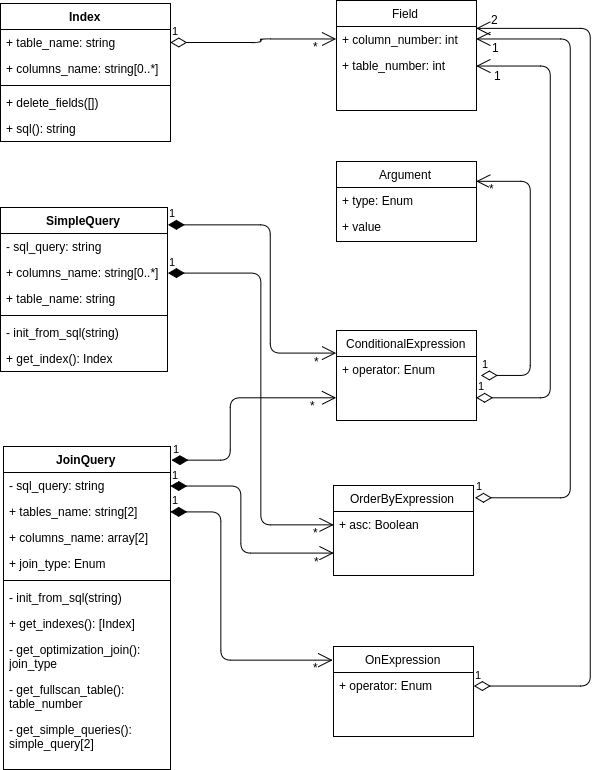
\includegraphics[scale=0.7]{diag-class.png}
  \caption{Диаграмма классов}
  \label{img:diag-class}
\end{figure}


\section{Тестирование разрбатываемого приложения}

Основываясь на виде запроса (листинг \ref{view-join-query}), который будет обрабатывать разрабатываемый инструмент, выделим параметры, которые могут изменяться и значения, которые они могут принимать (одно значение для каждого класса эквивалентности этого параметра):

\begin{enumerate}
\item \textbf{join}: \{left, right, inner\},
\item \textbf{where}: \{-, \textit{t1.a = const}, \textit{t2.a = const}, \textit{t1.a <> const}, \textit{t2.a <> const}\}
\item \textbf{order by}: \{-, t1.a, t2.a\}
\end{enumerate}

Учитывая колличество параметров и их значения, для тестрования разрабатываемого ПО необходимо провести $3 * 5 * 3 = 45$ экспериментов.

По \textit{методу всех пар}, т.к. большинство ошибок проявляются либо при конкретных значениях одного параметра, либо взаимным влиянием значений двух параметров \cite{article:Telcordia}, то достаточно провести 15 экспериментов. План экспериментов представлен в таблице \ref{table:list_experiments}.

\begin{table}[h]
\caption{План экспериментов}\label{table:list_experiments}.
\medskip
\begin{tabular}{|l|l|l|l|}
\hline
№ & join & order by & where\\
\hline
1 & inner & - & $-$\\\hline
2 & inner & t1.c & $t1.b = const$\\\hline
3 & inner & t2.c & $t2.b = const$\\\hline
4 & inner & - & $t1.b > const$\\\hline
5 & inner & t1.c & $t2.b > const$\\\hline
6 & left & t2.c & $-$\\\hline
7 & left & - & $t1.b = const$\\\hline
8 & left & t1.c & $t2.b = const$\\\hline
9 & left & t2.c & $t1.b > const$\\\hline
10 & left & - & $t2.b > const$\\\hline
11 & right & t1.c & $-$\\\hline
12 & right & t2.c & $t1.b = const$\\\hline
13 & right & - & $t2.b = const$\\\hline
14 & right & t1.c & $t1.b > const$\\\hline
15 & right & t2.c & $t2.b > const$\\\hline
\end{tabular}
\end{table}
